%!TeX root=../emmatop.tex
\chapter[Chapter \thechapter]{}
\lettrine[lraise=0.3]{H}{arriet} Smith's intimacy at Hartfield was soon a settled thing. Quick and decided in her ways, Emma lost no time in inviting, encouraging, and telling her to come very often; and as their acquaintance increased, so did their satisfaction in each other. As a walking companion, Emma had very early foreseen how useful she might find her. In that respect Mrs Weston's loss had been important. Her father never went beyond the shrubbery, where two divisions of the ground sufficed him for his long walk, or his short, as the year varied; and since Mrs Weston's marriage her exercise had been too much confined. She had ventured once alone to Randalls, but it was not pleasant; and a Harriet Smith, therefore, one whom she could summon at any time to a walk, would be a valuable addition to her privileges. But in every respect, as she saw more of her, she approved her, and was confirmed in all her kind designs.

Harriet certainly was not clever, but she had a sweet, docile, grateful disposition, was totally free from conceit, and only desiring to be guided by any one she looked up to. Her early attachment to herself was very amiable; and her inclination for good company, and power of appreciating what was elegant and clever, shewed that there was no want of taste, though strength of understanding must not be expected. Altogether she was quite convinced of Harriet Smith's being exactly the young friend she wanted—exactly the something which her home required. Such a friend as Mrs Weston was out of the question. Two such could never be granted. Two such she did not want. It was quite a different sort of thing, a sentiment distinct and independent. Mrs Weston was the object of a regard which had its basis in gratitude and esteem. Harriet would be loved as one to whom she could be useful. For Mrs Weston there was nothing to be done; for Harriet every thing.

Her first attempts at usefulness were in an endeavour to find out who were the parents, but Harriet could not tell. She was ready to tell every thing in her power, but on this subject questions were vain. Emma was obliged to fancy what she liked—but she could never believe that in the same situation \textit{she} should not have discovered the truth. Harriet had no penetration. She had been satisfied to hear and believe just what Mrs Goddard chose to tell her; and looked no farther.

Mrs Goddard, and the teachers, and the girls and the affairs of the school in general, formed naturally a great part of the conversation—and but for her acquaintance with the Martins of Abbey-Mill Farm, it must have been the whole. But the Martins occupied her thoughts a good deal; she had spent two very happy months with them, and now loved to talk of the pleasures of her visit, and describe the many comforts and wonders of the place. Emma encouraged her talkativeness—amused by such a picture of another set of beings, and enjoying the youthful simplicity which could speak with so much exultation of Mrs Martin's having <\textit{two} parlours, two very good parlours, indeed; one of them quite as large as Mrs Goddard's drawing-room; and of her having an upper maid who had lived five-and-twenty years with her; and of their having eight cows, two of them Alderneys, and one a little Welch cow, a very pretty little Welch cow indeed; and of Mrs Martin's saying as she was so fond of it, it should be called \textit{her} cow; and of their having a very handsome summer-house in their garden, where some day next year they were all to drink tea:—a very handsome summer-house, large enough to hold a dozen people.>

For some time she was amused, without thinking beyond the immediate cause; but as she came to understand the family better, other feelings arose. She had taken up a wrong idea, fancying it was a mother and daughter, a son and son's wife, who all lived together; but when it appeared that the Mr Martin, who bore a part in the narrative, and was always mentioned with approbation for his great good-nature in doing something or other, was a single man; that there was no young Mrs Martin, no wife in the case; she did suspect danger to her poor little friend from all this hospitality and kindness, and that, if she were not taken care of, she might be required to sink herself forever.

With this inspiriting notion, her questions increased in number and meaning; and she particularly led Harriet to talk more of Mr Martin, and there was evidently no dislike to it. Harriet was very ready to speak of the share he had had in their moonlight walks and merry evening games; and dwelt a good deal upon his being so very good-humoured and obliging. He had gone three miles round one day in order to bring her some walnuts, because she had said how fond she was of them, and in every thing else he was so very obliging. He had his shepherd's son into the parlour one night on purpose to sing to her. She was very fond of singing. He could sing a little himself. She believed he was very clever, and understood every thing. He had a very fine flock, and, while she was with them, he had been bid more for his wool than any body in the country. She believed every body spoke well of him. His mother and sisters were very fond of him. Mrs Martin had told her one day (and there was a blush as she said it,) that it was impossible for any body to be a better son, and therefore she was sure, whenever he married, he would make a good husband. Not that she \textit{wanted} him to marry. She was in no hurry at all.

<Well done, Mrs Martin!> thought Emma. <You know what you are about.>

<And when she had come away, Mrs Martin was so very kind as to send Mrs Goddard a beautiful goose—the finest goose Mrs Goddard had ever seen. Mrs Goddard had dressed it on a Sunday, and asked all the three teachers, Miss Nash, and Miss Prince, and Miss Richardson, to sup with her.>

<Mr Martin, I suppose, is not a man of information beyond the line of his own business? He does not read?>

<Oh yes!—that is, no—I do not know—but I believe he has read a good deal—but not what you would think any thing of. He reads the \textit{Agricultural Reports}, and some other books that lay in one of the window seats—but he reads all \textit{them} to himself. But sometimes of an evening, before we went to cards, he would read something aloud out of the \textit{Elegant Extracts}, very entertaining. And I know he has read \textit{The Vicar of Wakefield}. He never read \textit{The Romance of the Forest}, nor \textit{The Children of the Abbey}. He had never heard of such books before I mentioned them, but he is determined to get them now as soon as ever he can.>

The next question was—

<What sort of looking man is Mr Martin?>

<Oh! not handsome—not at all handsome. I thought him very plain at first, but I do not think him so plain now. One does not, you know, after a time. But did you never see him? He is in Highbury every now and then, and he is sure to ride through every week in his way to Kingston. He has passed you very often.>

<That may be, and I may have seen him fifty times, but without having any idea of his name. A young farmer, whether on horseback or on foot, is the very last sort of person to raise my curiosity. The yeomanry are precisely the order of people with whom I feel I can have nothing to do. A degree or two lower, and a creditable appearance might interest me; I might hope to be useful to their families in some way or other. But a farmer can need none of my help, and is, therefore, in one sense, as much above my notice as in every other he is below it.>

<To be sure. Oh yes! It is not likely you should ever have observed him; but he knows you very well indeed—I mean by sight.>

<I have no doubt of his being a very respectable young man. I know, indeed, that he is so, and, as such, wish him well. What do you imagine his age to be?>

<He was four-and-twenty the 8th of last June, and my birthday is the 23rd just a fortnight and a day's difference—which is very odd.>

<Only four-and-twenty. That is too young to settle. His mother is perfectly right not to be in a hurry. They seem very comfortable as they are, and if she were to take any pains to marry him, she would probably repent it. Six years hence, if he could meet with a good sort of young woman in the same rank as his own, with a little money, it might be very desirable.>

<Six years hence! Dear Miss Woodhouse, he would be thirty years old!>

<Well, and that is as early as most men can afford to marry, who are not born to an independence. Mr Martin, I imagine, has his fortune entirely to make—cannot be at all beforehand with the world. Whatever money he might come into when his father died, whatever his share of the family property, it is, I dare say, all afloat, all employed in his stock, and so forth; and though, with diligence and good luck, he may be rich in time, it is next to impossible that he should have realised any thing yet.>

<To be sure, so it is. But they live very comfortably. They have no indoors man, else they do not want for any thing; and Mrs Martin talks of taking a boy another year.>

<I wish you may not get into a scrape, Harriet, whenever he does marry;—I mean, as to being acquainted with his wife—for though his sisters, from a superior education, are not to be altogether objected to, it does not follow that he might marry any body at all fit for you to notice. The misfortune of your birth ought to make you particularly careful as to your associates. There can be no doubt of your being a gentleman's daughter, and you must support your claim to that station by every thing within your own power, or there will be plenty of people who would take pleasure in degrading you.>

<Yes, to be sure, I suppose there are. But while I visit at Hartfield, and you are so kind to me, Miss Woodhouse, I am not afraid of what any body can do.>

<You understand the force of influence pretty well, Harriet; but I would have you so firmly established in good society, as to be independent even of Hartfield and Miss Woodhouse. I want to see you permanently well connected, and to that end it will be advisable to have as few odd acquaintance as may be; and, therefore, I say that if you should still be in this country when Mr Martin marries, I wish you may not be drawn in by your intimacy with the sisters, to be acquainted with the wife, who will probably be some mere farmer's daughter, without education.>

<To be sure. Yes. Not that I think Mr Martin would ever marry any body but what had had some education—and been very well brought up. However, I do not mean to set up my opinion against yours—and I am sure I shall not wish for the acquaintance of his wife. I shall always have a great regard for the Miss Martins, especially Elizabeth, and should be very sorry to give them up, for they are quite as well educated as me. But if he marries a very ignorant, vulgar woman, certainly I had better not visit her, if I can help it.>

Emma watched her through the fluctuations of this speech, and saw no alarming symptoms of love. The young man had been the first admirer, but she trusted there was no other hold, and that there would be no serious difficulty, on Harriet's side, to oppose any friendly arrangement of her own.

\begin{figure}[tbph]
\centering
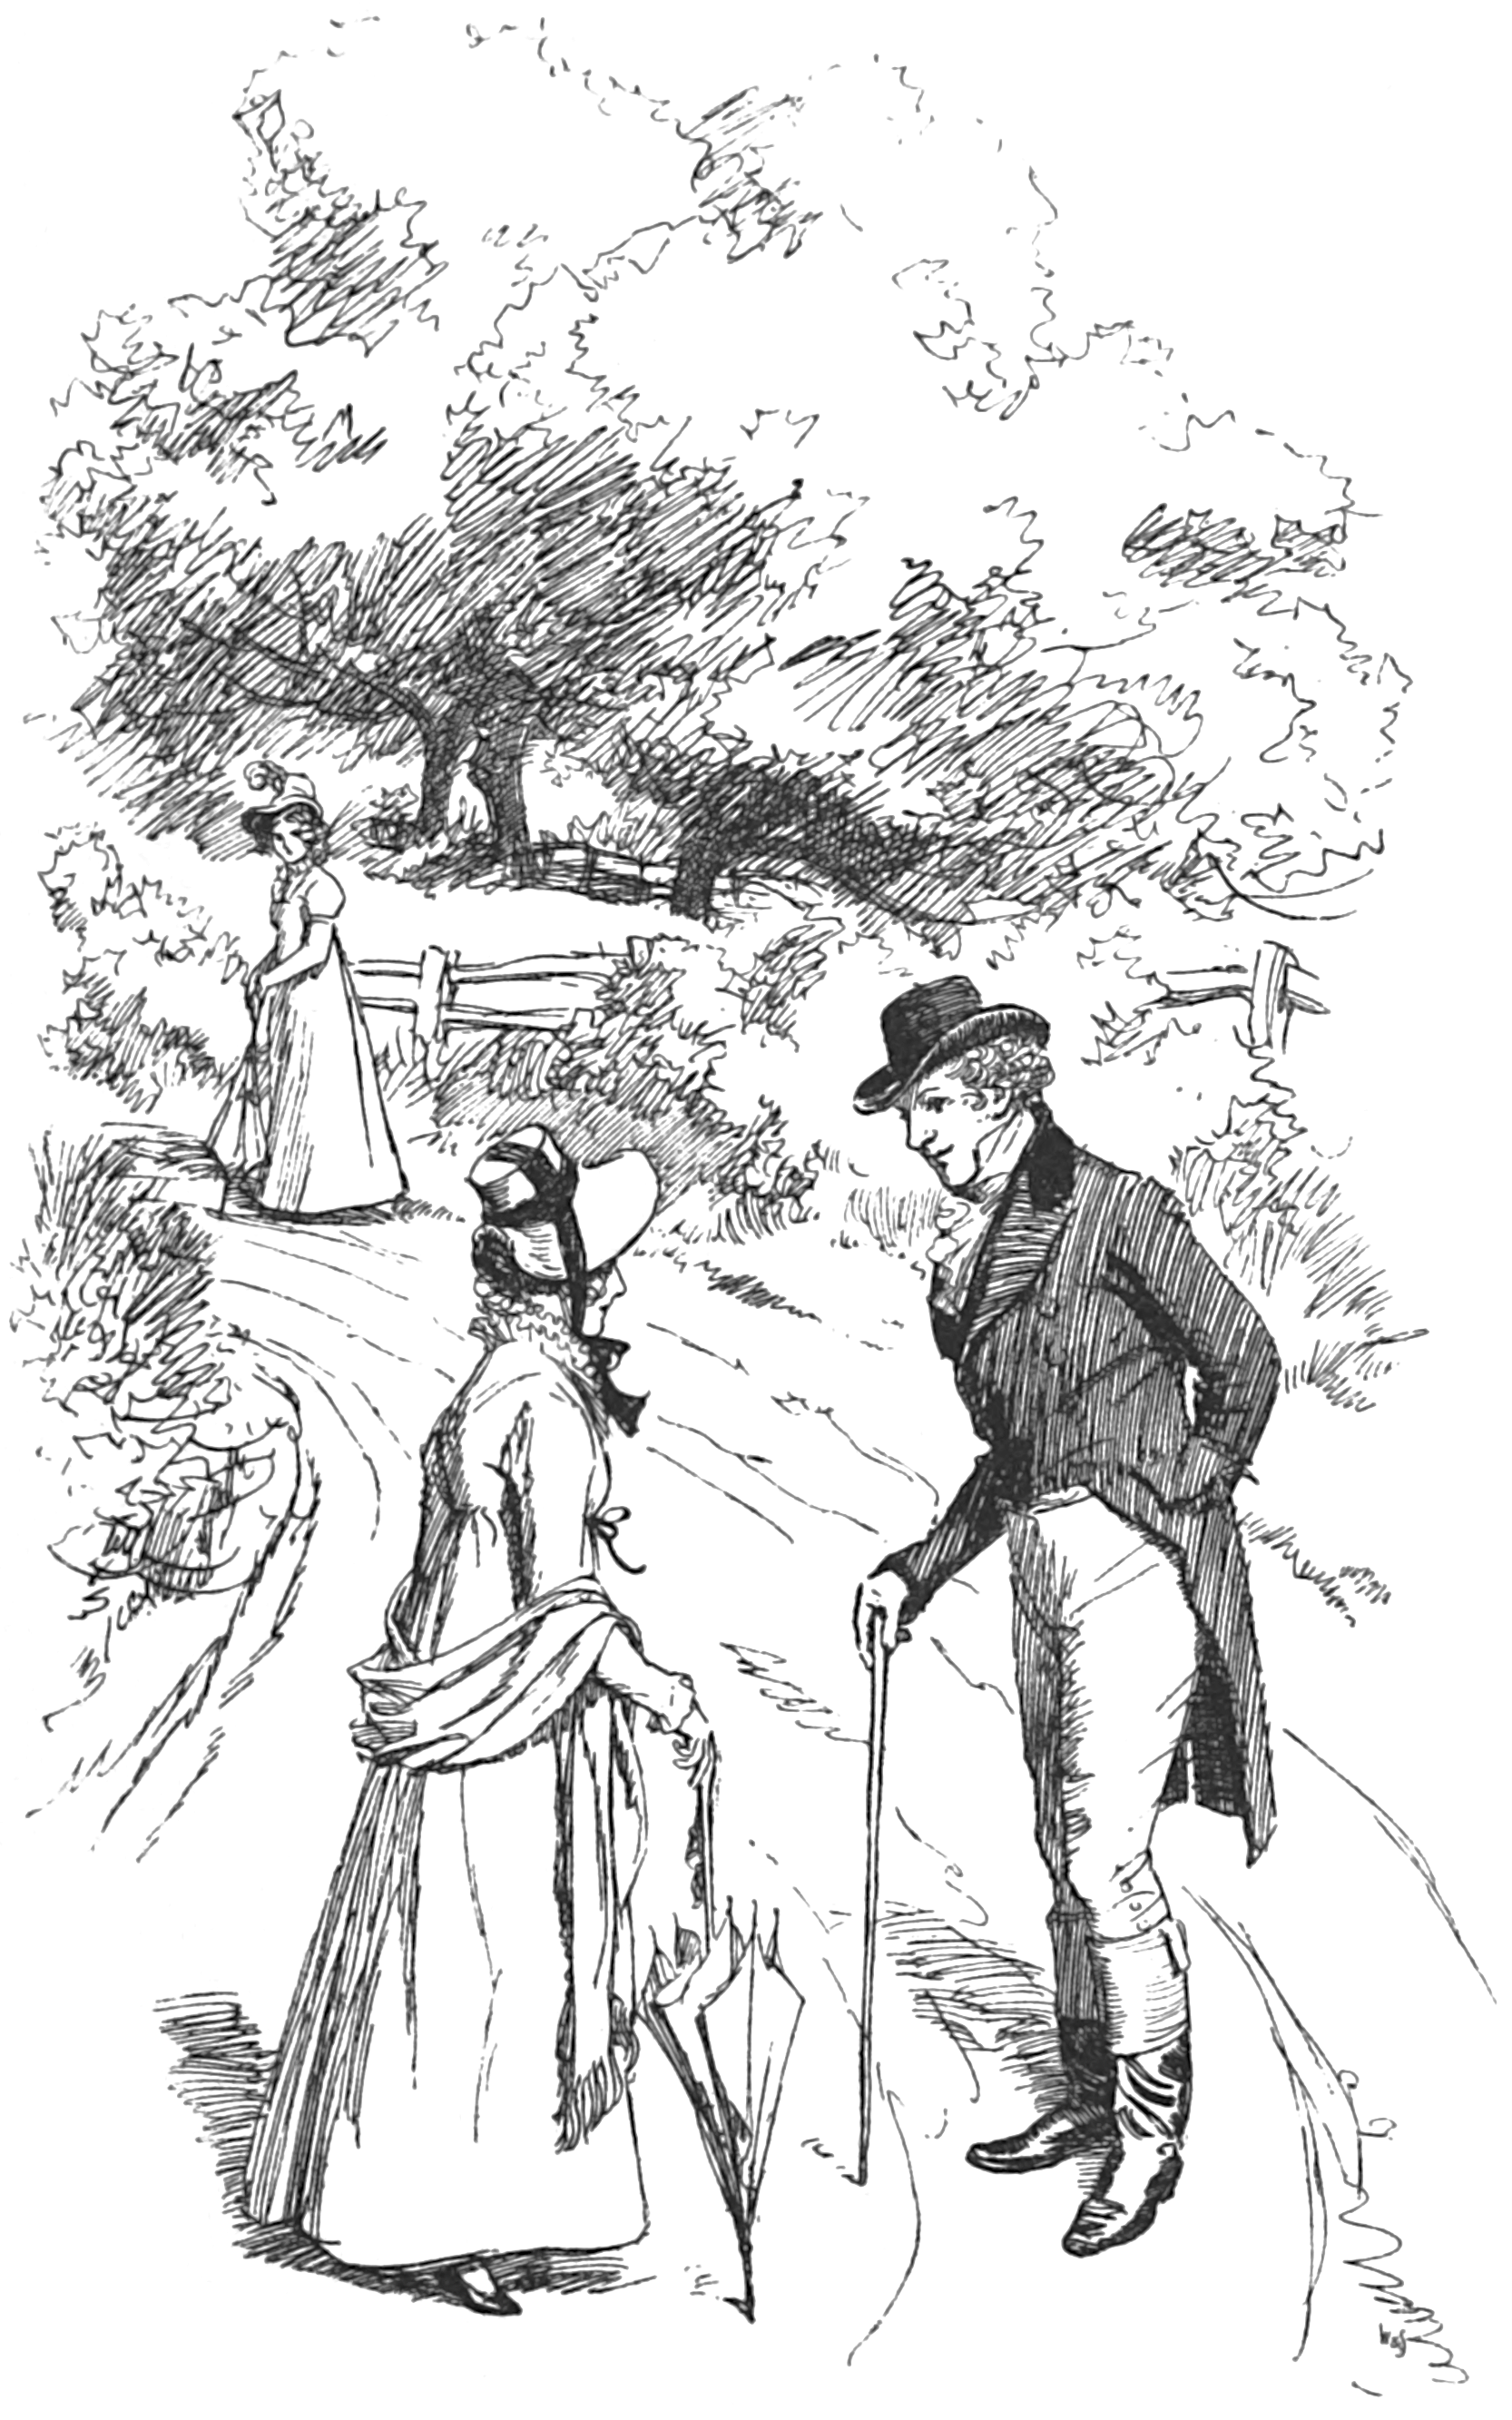
\includegraphics[width=.8\linewidth]{4notsorry}
\caption{Emma was not sorry to have such an opportunity of survey}
\end{figure}

They met Mr Martin the very next day, as they were walking on the Donwell road. He was on foot, and after looking very respectfully at her, looked with most unfeigned satisfaction at her companion. Emma was not sorry to have such an opportunity of survey; and walking a few yards forward, while they talked together, soon made her quick eye sufficiently acquainted with Mr Robert Martin. His appearance was very neat, and he looked like a sensible young man, but his person had no other advantage; and when he came to be contrasted with gentlemen, she thought he must lose all the ground he had gained in Harriet's inclination. Harriet was not insensible of manner; she had voluntarily noticed her father's gentleness with admiration as well as wonder. Mr Martin looked as if he did not know what manner was.

They remained but a few minutes together, as Miss Woodhouse must not be kept waiting; and Harriet then came running to her with a smiling face, and in a flutter of spirits, which Miss Woodhouse hoped very soon to compose.

<Only think of our happening to meet him!—How very odd! It was quite a chance, he said, that he had not gone round by Randalls. He did not think we ever walked this road. He thought we walked towards Randalls most days. He has not been able to get the Romance of the Forest yet. He was so busy the last time he was at Kingston that he quite forgot it, but he goes again to-morrow. So very odd we should happen to meet! Well, Miss Woodhouse, is he like what you expected? What do you think of him? Do you think him so very plain?>

<He is very plain, undoubtedly—remarkably plain:—but that is nothing compared with his entire want of gentility. I had no right to expect much, and I did not expect much; but I had no idea that he could be so very clownish, so totally without air. I had imagined him, I confess, a degree or two nearer gentility.>

<To be sure,> said Harriet, in a mortified voice, <he is not so genteel as real gentlemen.>

<I think, Harriet, since your acquaintance with us, you have been repeatedly in the company of some such very real gentlemen, that you must yourself be struck with the difference in Mr Martin. At Hartfield, you have had very good specimens of well educated, well bred men. I should be surprized if, after seeing them, you could be in company with Mr Martin again without perceiving him to be a very inferior creature—and rather wondering at yourself for having ever thought him at all agreeable before. Do not you begin to feel that now? Were not you struck? I am sure you must have been struck by his awkward look and abrupt manner, and the uncouthness of a voice which I heard to be wholly unmodulated as I stood here.>

<Certainly, he is not like Mr Knightley. He has not such a fine air and way of walking as Mr Knightley. I see the difference plain enough. But Mr Knightley is so very fine a man!>

<Mr Knightley's air is so remarkably good that it is not fair to compare Mr Martin with \textit{him}. You might not see one in a hundred with \textit{gentleman} so plainly written as in Mr Knightley. But he is not the only gentleman you have been lately used to. What say you to Mr Weston and Mr Elton? Compare Mr Martin with either of \textit{them}. Compare their manner of carrying themselves; of walking; of speaking; of being silent. You must see the difference.>

<Oh yes!—there is a great difference. But Mr Weston is almost an old man. Mr Weston must be between forty and fifty.>

<Which makes his good manners the more valuable. The older a person grows, Harriet, the more important it is that their manners should not be bad; the more glaring and disgusting any loudness, or coarseness, or awkwardness becomes. What is passable in youth is detestable in later age. Mr Martin is now awkward and abrupt; what will he be at Mr Weston's time of life?>

<There is no saying, indeed,> replied Harriet rather solemnly.

<But there may be pretty good guessing. He will be a completely gross, vulgar farmer, totally inattentive to appearances, and thinking of nothing but profit and loss.>

<Will he, indeed? That will be very bad.>

<How much his business engrosses him already is very plain from the circumstance of his forgetting to inquire for the book you recommended. He was a great deal too full of the market to think of any thing else—which is just as it should be, for a thriving man. What has he to do with books? And I have no doubt that he \textit{will} thrive, and be a very rich man in time—and his being illiterate and coarse need not disturb \textit{us}.>

<I wonder he did not remember the book>—was all Harriet's answer, and spoken with a degree of grave displeasure which Emma thought might be safely left to itself. She, therefore, said no more for some time. Her next beginning was,

<In one respect, perhaps, Mr Elton's manners are superior to Mr Knightley's or Mr Weston's. They have more gentleness. They might be more safely held up as a pattern. There is an openness, a quickness, almost a bluntness in Mr Weston, which every body likes in \textit{him}, because there is so much good-humour with it—but that would not do to be copied. Neither would Mr Knightley's downright, decided, commanding sort of manner, though it suits \textit{him} very well; his figure, and look, and situation in life seem to allow it; but if any young man were to set about copying him, he would not be sufferable. On the contrary, I think a young man might be very safely recommended to take Mr Elton as a model. Mr Elton is good-humoured, cheerful, obliging, and gentle. He seems to me to be grown particularly gentle of late. I do not know whether he has any design of ingratiating himself with either of us, Harriet, by additional softness, but it strikes me that his manners are softer than they used to be. If he means any thing, it must be to please you. Did not I tell you what he said of you the other day?>

She then repeated some warm personal praise which she had drawn from Mr Elton, and now did full justice to; and Harriet blushed and smiled, and said she had always thought Mr Elton very agreeable.

Mr Elton was the very person fixed on by Emma for driving the young farmer out of Harriet's head. She thought it would be an excellent match; and only too palpably desirable, natural, and probable, for her to have much merit in planning it. She feared it was what every body else must think of and predict. It was not likely, however, that any body should have equalled her in the date of the plan, as it had entered her brain during the very first evening of Harriet's coming to Hartfield. The longer she considered it, the greater was her sense of its expediency. Mr Elton's situation was most suitable, quite the gentleman himself, and without low connexions; at the same time, not of any family that could fairly object to the doubtful birth of Harriet. He had a comfortable home for her, and Emma imagined a very sufficient income; for though the vicarage of Highbury was not large, he was known to have some independent property; and she thought very highly of him as a good-humoured, well-meaning, respectable young man, without any deficiency of useful understanding or knowledge of the world.

She had already satisfied herself that he thought Harriet a beautiful girl, which she trusted, with such frequent meetings at Hartfield, was foundation enough on his side; and on Harriet's there could be little doubt that the idea of being preferred by him would have all the usual weight and efficacy. And he was really a very pleasing young man, a young man whom any woman not fastidious might like. He was reckoned very handsome; his person much admired in general, though not by her, there being a want of elegance of feature which she could not dispense with:—but the girl who could be gratified by a Robert Martin's riding about the country to get walnuts for her might very well be conquered by Mr Elton's admiration.